\chapter{Link Discovery}

Das folgende Kapitel beschäftigt sich mit den im Rahmen dieser Arbeit unternommenen Schritten zur Link Discovery, also dem Finden von Beziehungen zwischen Wörtern und Wortgruppen. Dazu zählen die Generierung eines Ausgangsgraphen aus Tag-Daten sowie dessen Anreicherung durch die Integration weiterer interner und externer Datenquellen.

\section{Tags}

Den Ausgangspunkt für den in \ref{solution} beschriebenen Lösungsansatz stellen die Daten des Tag-Systems dar. Diese werden in \ref{tag-system} ausführlich beschrieben. Aus diesen Daten wird im ersten Schritt der Graph erstellt, in diesen in allen weiteren Schritten weitere Daten integriert werden. Die in diesem Graph enthaltenen Knoten stellen also die Kriterien für die Abfrage der weiteren Datenquellen dar.

Um den Ausgangsgraphen zu berechnen, sind die Schritte des Imports, der Bereinigung, der Reduktion, der Transformation und der Integration notwendig \cite{hkp2012}, welche im folgenden genauer beschrieben werden.

\subsection{Import}

Die Daten liegen im Quellsystem in relationaler Form vor. Somit existieren Tabellen für die Tags, Dokumente und Verknüpfungen zwischen ebenjenen. Da der Inhalt der Dokumente nicht relevant für die Link Discovery mittels Kookkurenz sind, genügt es, die Tabellen der Tags und Verknüpfungen zu importieren.

Die Tags liegen in der Form \((i, s, l)\) vor, wobei \(i\) den eindeutigen Bezeichner des Tags, \(s\) die Zeichenkette und \(l\) die Sprache des Tags repräsentieren.

Die Verknüpfungen sind durch Tupel der Form \((i, t, d_t, d_i)\) repräsentiert, wobei \(i\) der eindeutige Bezeichner der Verknüpfung selbst ist. \(t\) ist der Bezeichner des Tags, \(d_t\) der Typ des Dokuments und \(d_i\) der Bezeichner des Dokumentes. \(d_t\) und \(d_i\) bilden also den zusammengesetzten Schlüssel des getaggten Dokumentes. 
 
\begin{figure}
\label{fig:tag_source_erd}
\begin{center}
    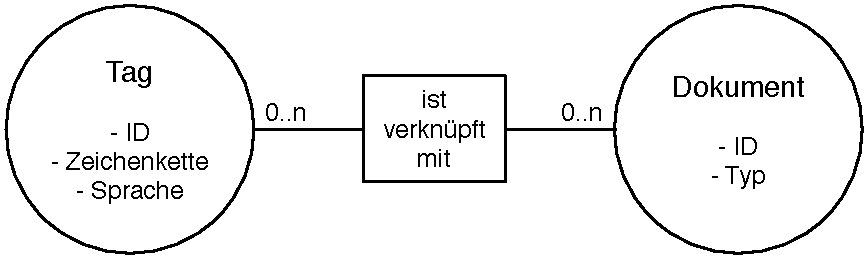
\includegraphics[width=0.6\textwidth]{tag_source_erd}
\end{center}
\caption{Tag-Quelldaten als Entity-Relationship Diagramm}
\end{figure}

Die importierten Quelldaten sind in Abbildung \ref{fig:tag_source_erd} als Entity - Relationship Diagramm abgebildet. Nach dem Import stehen \num{2072079} Tags und \num{71938905} Verknüpfungen zur Verfügung.

\subsection{Bereinigung}

An den Tag-Daten liegen die in \ref{quality} genannten Defekte in Hinblick auf die Datenqualität vor. Diese sollten in einem Bereinigungsschritt reduziert werden. Hierbei liegt das Hauptaugenmerk auf der Erkennung von Duplikaten und später nicht verwertbaren Zeichenketten. Alle durchgeführten Maßnahmen zur Bereinigung beziehen sich hierbei auf die Eigenschaft \(s\) des Tags, also der Zeichenkette selbst.

In den unbereinigten importierten Daten existieren keine Duplikate in der Art, dass eine Paarung aus Zeichenkette und Sprache immer nur genau einmal in den Daten vorhanden ist. Jedoch enthalten viele der Tags nicht weiter verwertbare Zeichen wie nicht druckbare ASCII Zeichen, Anführungszeichen, Satzzeichen, Sonderzeichen sowie überflüssige Leerzeichen am Anfang und Ende der Zeichenkette. Außerdem existiert in den importierten Daten eine Unterscheidung zwischen Groß- und Kleinschreibung. Diese Unterscheidung bringt im Kontext der Link Discovery keine Vorteile und kann somit entfernt werden.

\begin{table}
\centering
\begin{tabular}{|l|l|}
    \hline
    Rohdaten & Bereinigte Daten \\
    \hline
    \textbackslash u0003\textbackslash r\textbackslash nregenbogen & regenbogen \\
    RegenBogen & regenbogen \\
    "Regenbogen" & regenbogen \\
    regenbogen +einhorn & regenbogen einhorn\\
    \hspace{10 mm} regenbogen & regenbogen \\
    regenbogen & regenbogen \\
    \hline
\end{tabular}
\caption{Beispiele für die Tag-Bereinigung}
\label{tab:tag_cleaning}
\end{table}

Somit besteht der Bereinigungsschritt darin, nicht verwertbare Zeichen zu entfernen und alle Großbuchstaben in Kleinbuchstaben umzuwandeln. Dadurch entstehen Duplikate, welche im darauf folgenden Reduktionsschritt entfernt werden können. In Tabelle \ref{tab:tag_cleaning} sind einige Beispiele für die Bereinigungen aufgeführt. Dabei ist gut zu erkennen, dass durch die Bereinigungen Duplikate erzeugt werden.

\subsection{Reduktion}

Der Reduktionsschritt dient zur Einschränkung der Gesamtdaten auf eine nützliche oder handhabbare Menge. Außerdem kann durch Reduktion auch die Datenqualität verbessert werden.

Im Fall der Tag-Daten liegt das Hauptaugenmerk im Reduktionsschritt auf der Entfernung von Duplikaten, die bei der Bereinigung entstanden sind. Dabei muss gleichzeitig sicher gestellt werden, dass keine Informationen über die Verwendung der Tags verloren gehen. Somit besteht die Duplikatentfernung der Tags im Zusammenführen von Datensätzen mit gleichen Zeichenketten und Sprachen. Dabei werden auch die Verwendungen der Tags zusammengeführt.

Werden die Verknüpfungen zweier Tags mit Dokumenten zusammengeführt, können auch dabei wieder Duplikate entstehen. Diese müssen in diesem Fall entfernt werden, da ein Tag nicht mehrmals mit einem Dokument verknüpft werden kann. Das Zusammenfühen von Tags ist exemplarisch in Abbildung \ref{fig:tag_reduction} dargestellt.

\begin{figure}
\label{fig:tag_reduction}
\begin{center}
    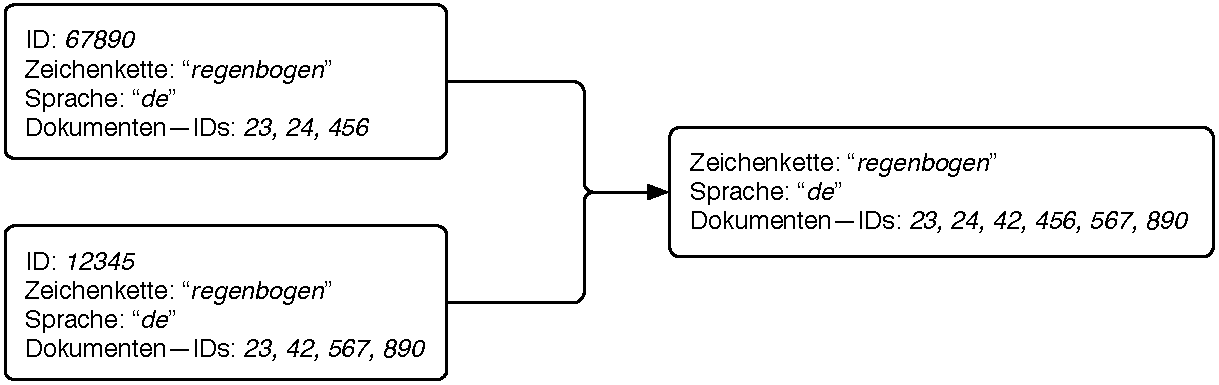
\includegraphics[width=0.7\textwidth]{tag_reduction}
\end{center}
\caption{Beispiel für das Zusammenführen der bereinigten Tags}
\end{figure}

Eine weitere im Rahmen dieser Arbeit unternommene Maßnahme zur Datenreduktion bestand darin, sich auf die Menge der Tags zu beschränken, deren Attribut \(l\) den Wert \emph{de} besitzt. Praktisch handelt es sich dabei um alle Tags, die als deutsch gekennzeichnet in der Datenbank gespeichert sind. Diese Einschränkung wurde vorgenommen, um die zu verarbeitende Datenmenge überschaubar zu halten.

Ein letzter Reduktionsschritt besteht in der Entfernung der Tags, deren Zeichenketten eine Länge von \num{1} besitzen, da in der deutschen Sprache keine einbuchstabigen Wörter existieren.

Nach der beschriebenen Reduktion befinden sich noch \num{314351} Tags und \num{23255714} Verknüpfungen in der Datenbank. Dies entspricht einer Reduktion von ca. \num{68} Prozent gegenüber der importierten Menge von Objekten.

\subsection{Transformation}

Der Transformationsschritt beschreibt die Überführung der Daten in die Form, die für das Ergebnis benötigt wird. Im Falle der Tag-Daten bedeutet dies eine Umformung in die Form des Kokkurrenzgraphen, also die Erzeugung von Knoten- und Kantenobjekten. Die Umsetzung dieser Transformation mittels des Programmiermodells MapReduce wurde in \ref{mapreduce_cooccurence} genauer beschrieben.

Um die vorhandenen Informationen später einfach nutzbar zu machen, erscheint es sinnvoll, die Knoten mit allen verfügbaren Daten anzureichern. Dazu gehören bei den Tags die Sprache und Zeichenkette, sowie Informationen darüber an welche Dokumente der Tag verwendet wurde. Diese Informationen lassen sich in einer dokumentenbasierten Datenbank leicht abbilden.

Je Tag wird ein Datenbankdokument erzeugt, dass den Knoten repräsentiert. Dieses besitzt als Attribute zum einen die Zeichenkette und die Sprache des Tags, aus dem es erzeugt wurde. Zum anderen wird ein Unterdokument hinzugefügt, welches weitere Eigenschaften des Ausgangstags beschreibt. Die umfasst die Anzahl der Verwendungen und die eindeutigen Bezeichner der Dokumente, die mit dem Tag getaggt wurden. Außerdem kann im Transformationsschritt für jeden Knoten ein global eindeutiger Bezeichner erzeugt werden, um das spätere Referenzieren der Knoten einfacher zu machen. Zeichenkette und Sprache des Knotens stellen einen zusammengesetzten Schlüssel dar und sind in der Knotenmenge eindeutig. Der Aufbau der Knoten ist schemahaft in Abbildung \ref{fig:tag_transform_node} dargestellt.

\begin{figure}
\label{fig:tag_transform_node}
\begin{center}
    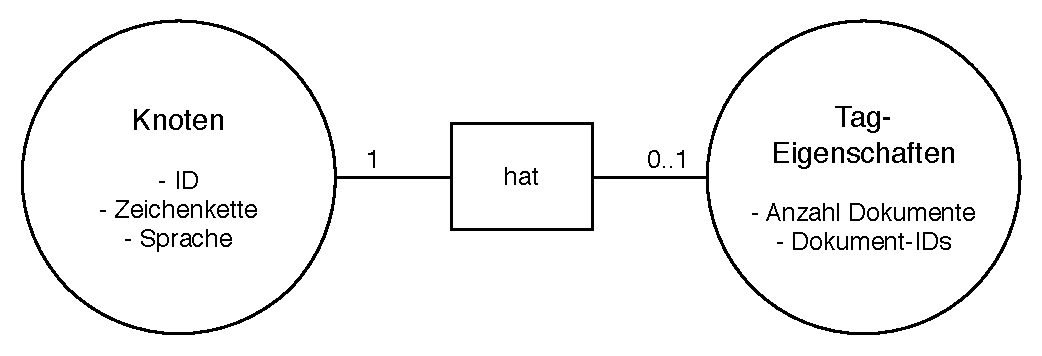
\includegraphics[width=0.7\textwidth]{tag_transform_node}
\end{center}
\caption{Aufbau der aus den Tag-Daten erzeugten Knoten}
\end{figure}

Die Erzeugung der Kanten erfolgt dann wie in Abschnitt \ref{mapreduce_cooccurence} beschrieben. Dabei werden für jedes gemeinsame Auftreten von zwei Tags zwei Datenbankdokumente erzeugt. Dieses beschreiben gerichtete Kanten zwischen den Tags, die ein gemeinsames Auftreten der Tags repräsentieren. Neben Quell- und Zielknoten enthält eine Kante den Kantentyp sowie weitere Informationen über die Art der Verbindung. Im Fall von Kookkurenzkanten ist dies zum einen die absolute Anzahl gemeinsamer Vorkommen der Tags, zum anderen die in \ref{measures} beschriebenen Kookkurenzmaße. Der Kantentyp ist aus der Berechnung folgend der Typ der Tag-Kookkurenz. Der Aufbau der erzeugten Kanten ist in Abbildung \ref{fig:tag_transform_edge} dargestellt.

\begin{figure}
\label{fig:tag_transform_edge}
\begin{center}
    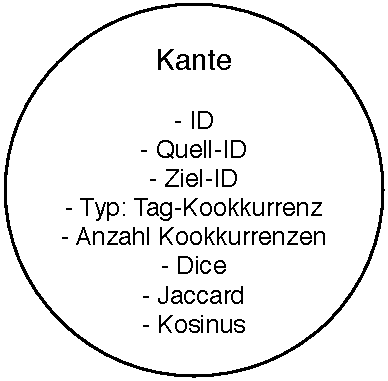
\includegraphics[width=0.3\textwidth]{tag_transform_edge}
\end{center}
\caption{Aufbau der aus den Tag-Daten erzeugten Kanten}
\end{figure}

\subsection{Integration}

\section{Clicktracking}

\section{Google Translate}

Google bietet im Rahmen seines \emph{Translate}-Services \cite{gt2013} eine kostenpfichtige API für Spracherkennung an. Diese ermöglicht es, die Sprache beliebiger Zeichenketten automatisch erkennen zu lassen. Google stellt hierzu eine REST-API zur Verfügung.

Diese Schnittstelle liefert Ergebnisse der Form \((l, c)\), wobei \(l\) die für die Zeichenkette erkannte Sprache und \(c\) einen Konfidenzwert für die Spracherkennung repräsentiert. Der Konfidenzwert liegt dabei im Intervall zwischen \num{0} und \num{1} und stellt die Verlässlichkeit der Spracherkennung dar.

Die Integration der Spracherkennungs-Daten in den Graphen gestaltet sich einfach. Dazu werden die durch die bereits vorhandenen Knoten repräsentierten Zeichenketten extrahiert und als Eingabedaten für die Spracherkennungs-API verwendet. Die Ergebnisse werden abgespeichert, um weitere kostenpflichtige Abfragen zu vermeiden.

Eine Bereinigung der Ergebnisse ist nicht erforderlich. Somit müssen die Ergebnisse lediglich in den Ausgangsgraphen integriert werden. Die Spracherkennung an sich bringt keine Ähnlichkeitsbeziehungen mit sich, sondern verbessert gegebenenfalls nur die Knotenauswahl für spätere Operationen.

In der Konsequenz genügt es also, die für die Abfrage verwendeten Knoten mit den Ergbenissen der Spracherkennung zu annotieren. Somit kann dann bei späteren Analysen anhand des Konfidenzwertes abgewogen werden, ob die erkannte Sprache oder die eventuell schon am Knoten vorhandene Sprache verwendet werden soll.

\section{Zerlegung von Wortgruppen}

\section{Wortschatz der Universität Leipzig}

Die Universität Leipzig betreibt ein Wortschatz-Projekt \cite{ws2013}. Im Rahmen dieses Projektes wird durch die Analyse von großen Textmengen eine Datenbank deutscher Wörter, deren Bedeutungen, grammatikalische Eigenschaften und Beziehungen zu anderen Wörtern aufgebaut.